\chapter{DESAIN DAN PERANCANGAN}
    Pada bab ini dibahas mengenai analisis dan perancangan sistem.
	
    \section{Kasus Penggunaan}
    	Terdapat dua aktor dalam sistem ini, yaitu Pengembang (Administrator) dan \textit{User} (Pengguna) dari aplikasi web yang dikelola oleh sistem. Diagram kasus penggunaan digambarkan pada Gambar \ref{usecase}.
        \begin{figure}[H]
			\centering
			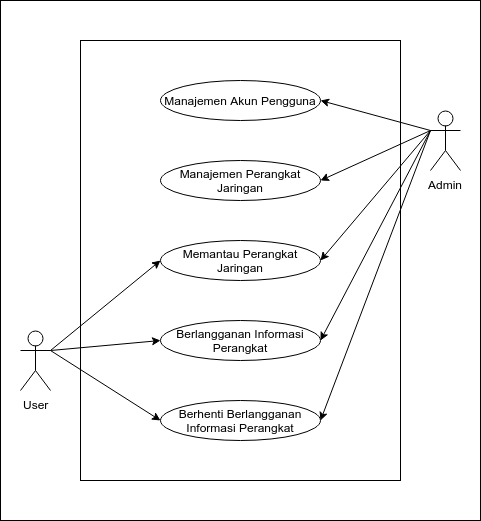
\includegraphics[width=8cm,height=10cm]{Images/C-3/usecase.png}
			\caption{Diagram Kasus Penggunaan}
			\label{usecase}
		\end{figure}
        \indent Diagram kasus penggunaan pada Gambar \ref{usecase} dideskripsikan masing-masing pada Tabel \ref {tabelKodeKasusPenggunaan}.
        
        \begin{longtable}{|p{0.25\textwidth}|p{0.24\textwidth}|p{0.35\textwidth}|} % L = Rata kiri untuk setiap kolom, | = garis batas vertikal.
		    	
		    	% Kepala tabel, berulang di setiap halaman
		    	\caption{Daftar Kode Kasus Penggunaan} \label{tabelKodeKasusPenggunaan} \\
		    	\hline
		    	\textbf{Kode Kasus Penggunaan} & \textbf{Nama Kasus Penggunaan} & \textbf{Keterangan} \\ \hline
		    	\endhead
		    	\endfoot
		    	\endlastfoot
		    	UC-0001 & Manajemen Akun Pengguna. & Pengembang (Admin) dapat membuat, melihat, mengubah dan menghapus data akun pengguna. \\ \hline
		    	UC-0002 & Manajemen Perangkat Jaringan.  & Pengembang (Admin) dapat membuat, melihat, mengubah dan menghapus data perangkat jaringan.\\ \hline
		    	UC-0003 & Memantau Perangkat Jaringan. & Pengembang (Admin) dan Pengguna (User) dapat memantau seluruh perangkat jaringan yang sudah ia langgani. \\ \hline
		    	UC-0004 & Berlangganan Informasi Perangkat. & Pengembang (Admin) dan Pengguna (User) dapat berlangganan informasi perangkat jaringan yang diinginkan. \\ \hline
		    	UC-0005 & Berhenti Berlangganan Informasi Perangkat. & Pengembang (Admin) dan Pengguna (User) dapat berhenti berlangganan informasi perangkat jaringan yang diinginkan. \\ \hline	
		    \end{longtable}

	\section{Arsitektur Sistem}
		Pada sub-bab ini, dibahas mengenai tahap analisis dan kebutuhan bisnis dan desain dari sistem yang akan dibangun.

		\subsection{Desain Umum Sistem}
			Sistem yang akan dibuat yaitu sistem yang dapat melakukan pemantauan pada perangkat jaringan yang berbasis \textit{web} dengan metode \textit{pusblish/subscribe}, dimana pengguna (\textit{user}) harus berlangganan kepada suatu informasi untuk mendapatkan informasi yang diinginkan.
			
			Sistem ini melibatkan 3 (Tiga) server yang berfungsi sebagai web server dan 1 (satu) server yang berfungsi sebagai database server. Server aplikasi dan websocket server berada pada satu server, sehingga pada implementasinya webserver aplikasi dan websocket dijalankan pada port yang berbeda. Pada sistem ini \textit{client} yaitu pengguna (\textit{user}) dan pengelola (\textit{admin}) akan mengakses aplikasi menggunakan web browser. yang nantinya jika mengakses fitur selain memantau perangkat jaringan, aplikasi akan mengirimkan \textit{request} HTTP kepada REST API, dimana REST API tersebut melakukan transaksi data kepada database server. setelah itu REST API akan mengirimkan \textit{response} kepada aplikasi.
			
			jika client mengakses fitur memantau jaringan, maka aplikasi akan terhubung dengan websocket yang tugasnya mengakses data yang berada pada pub/sub server, dimana pubsub server menyimpan data yang diterbitkan oleh nagios, data tersebut adalah hasil response SNMP nagios kepada tiap perangkat jaringan terkait.
			Penjelasan secara umum arsitektur sistem akan diuraikan pada Gambar \ref{DesainUmumSistem}.
            \begin{figure}[H]
				\centering
				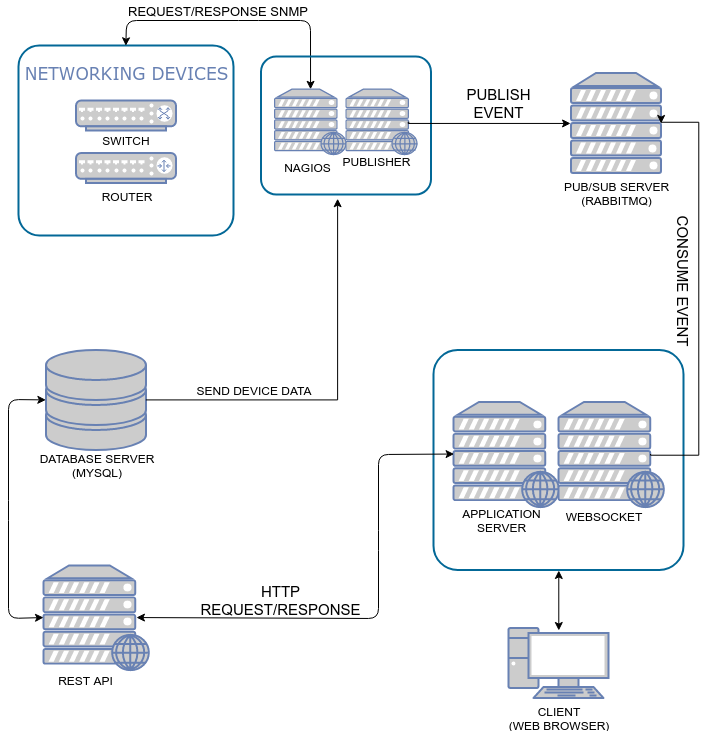
\includegraphics[width=9cm,height=8cm]{Images/C-3/main.png}
				\caption{Desain Umum Sistem}
				\label{DesainUmumSistem}
			\end{figure}

		\subsection{Desain REST API}
            	REST API bertujuan untuk menjadikan sistem yang memiliki performa yang baik, cepat dan mudah untuk di kembangkan (scale) terutama dalam pertukaran dan komunikasi data. REST API diakses menggunakan protokol HTTP. Penamaan dan struktur URL yang konsisten akan menghasilkan API yang baik dan mudah untuk dimengerti developer. URL API biasa disebut endpoint dalam pemanggilannya.
            	
            	Pada sistem ini terdapat beberapa endpoint, beberapa endpoint dibagi menjadi beberapa endpoint sesuai dengan perintah yang diajalankannya. misal: create, read, delete, update dan lain-lain. berikut ini adalah daftar endpoint yang dibutuhkan pada sistem ini:
            	\begin{enumerate}
            		\item "/"
            		\item "/register"
            		\item "/login"
					\item "/logout"
					\item "/users"
					\begin{enumerate}
						\item "/users/<id:string>"
						\item "/users/edit"
						\item "/users/delete"
					\end{enumerate}
					\item "/devices"
					\begin{enumerate}
						\item "/devices/<id:string>"
						\item "/devices/create"
						\item "/devices/edit"
						\item "/devices/delete"
					\end{enumerate}
					\item "/oid"
					\begin{enumerate}
						\item "/oid/create"
						\item "/oid/edit"
						\item "/oid/delete"
					\end{enumerate}
					\item "/subscribe"
					\begin{enumerate}
						\item "/subscribe/devices"
						\item "/subscribe/oid"
					\end{enumerate}
					\item "/unsubscribe"
					\begin{enumerate}
						\item "/unsubscribe/devices"
						\item "/unsubscribe/oid"
					\end{enumerate}           		
            	\end{enumerate}
            	
            	Server aplikasi mengirimkan HTTP request kepada REST API yang nantinya REST API akan melakukan trasaksi data pada database sesuai dengan endpointnya masing-masing. setelah itu REST API akan mengirimkan HTTP response kepada server aplikasi.
            	
            	Secara umum, arsitektur dari REST API dapat dilihat pada Gambar \ref{desain:desainrestapi}\\
                \begin{figure}[H]
                    \centering
                    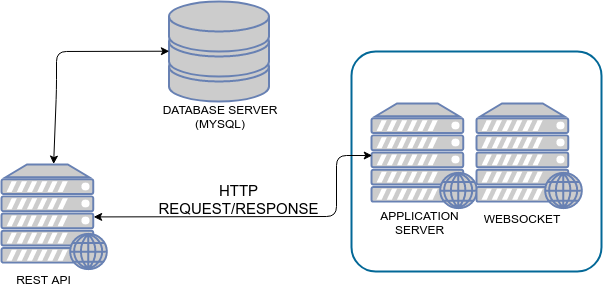
\includegraphics[width=9cm]{Images/C-3/desainrestapi.png}
                    \caption{Desain REST API}
                    \label{desain:desainrestapi}
				\end{figure}
            
		\subsection{Desain Publisher Server}
			Pada publisher server, dipasang aplikasi untuk memantau kinerja jaringan, yaitu Nagios. Pada nagios, perdapat plugin untuk memantau kinerja jaringan dengan protokol SNMP yaitu check-snmp. plugin ini membutuhkan beberapa parameter, diantaranya: alamat perangkat yang ingin dipantau dan oid dari apa yang ingin dipantau.
			
			Sebuah script dibuat untuk mengambil data dan mengirimkannya menuju pub/sub server. setiap perangkat yang dipantau dimasukkan ke sebuah thread baru agar dapat berjalan secara paralel. didalam thread tersebut, setiap perangkat terkait diperiksa kinerjanya dengan protokol SNMP dan hasilnya dikirimkan kepada pub/sub server melalui sebuah exchange yang telah diikat dengan sebuah message queue yang sebelumnya telah diinisiasi. Rancangan umum dari \textit{Publisher Server} seperti yang digambarkan pada Gambar \ref{desain:desainpublisher}.
			
			Exchange yang dibuat oleh script tersebut namanya dibuat berdasarkan uuid versi 4 dari tiap device yang diambil dari database dan nama queue dibuat berdasarkan uuid versi 4 yang dibuat baru.
			
			\begin{figure}[H]
				\centering
				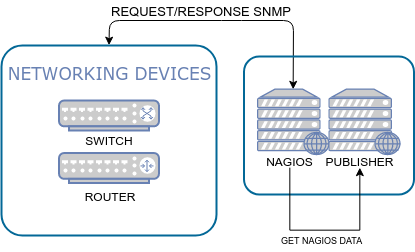
\includegraphics[width=9cm]{Images/C-3/desainpublisher.png}
				\caption{Desain Publisher Server}
				\label{desain:desainpublisher}
			\end{figure}
                
		\subsection{Desain Pub/Sub Server}
			Publish/subscribe server atau bisa juga disebut pub/sub server. yaitu sebuah server untuk menampung seluruh pesan yang dikirimkan oleh publisher. didalamnya terpasang aplikasi message broker yaitu RabbitMQ. seluruh pesan yang dikirimkan oleh publisher dikirimkan ke pub/sub server melalui sebuah exchange yang diikat dengan sebuah queue setelah itu server akan menyimpan pesan queue tersebut hingga ada consumer yang meminta data tersebut untuk dikirimkan. dalam kasus ini yang bertindak sebagai consumer adalah websocket server.
			
			Di sisi websocket dan server aplikasi, websocket menginisiasi sebuah exchange yang namanya dibuat berdasarkan uuid versi 4 dari tiap perangkat yang ingin dipantau dari database server, dengan syarat exchange dengan nama tersebut belum dibuat atau terdaftar sebelumnya. jika exchange dengan nama tersebut sudah dibuat atau terdaftar sebelumnya pada server maka websocket server tidak perlu membuat exchange tersebut. begitu juga dengan queue-nya. queue dibuat dengan nama uuid yang telah dibuat acak oleh client dengan algoritma uuid versi 4. setelah itu websocket baru mengambil data pereangkat sesuai dengan data apa saja yang dilanggani oleh client.
        	Secara umum, arsitektur rancangan dari \textit{Pub/Sub Server} dapat dilihat pada Gambar \ref{desain:desainpubsub}.
        	\begin{figure}[H]
				\centering
				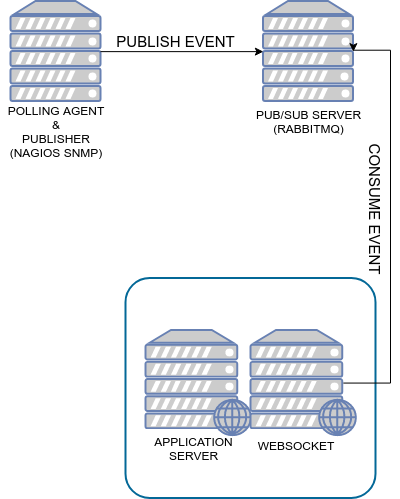
\includegraphics[width=7cm,height=7cm]{Images/C-3/desainpubsub.png}
				\caption{Desain Pub/Sub Server}
				\label{desain:desainpubsub}
			\end{figure}
            

        \subsection{Desain Database Server}
        	\begin{figure}[H]
        		\centering
        		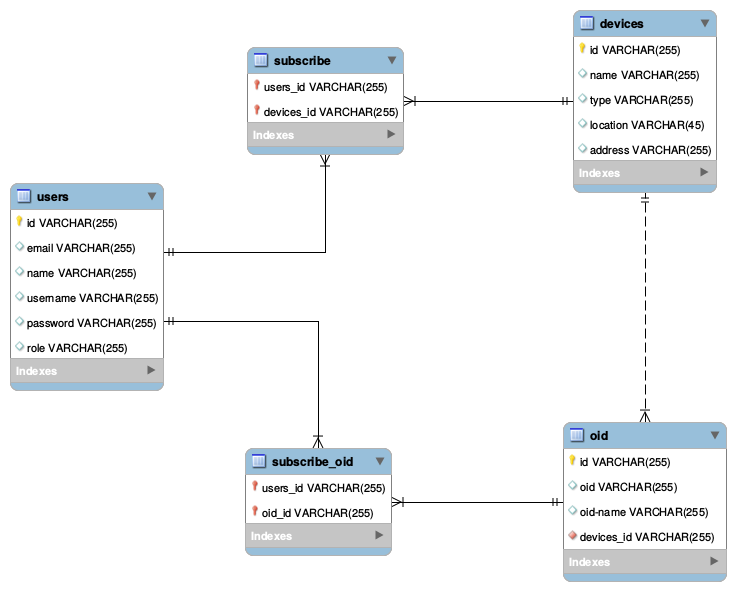
\includegraphics[width=9cm]{Images/C-3/desaindb.png}
        		\caption{Desain Database}
        		\label{desain:desaindatabase}
        	\end{figure}
        	
        	Desain database pada sistem ini adalah seperti yang digambarkan pada gambar \ref{desain:desaindatabase}. Terdapat tiga tabel utama yang mewakili tiap entitas yang terlibat dalam sistem ini, yaitu: users, devices, dan oid. selain itu, terdapat dua table many-to-many untuk menyimpan data pengguna yang telah berlangganan kepada tiap perangkat dan pengguna yang berlangganan kepada tiap OID (untuk mengetahui informasi apa saja yang ada pada tiap perangkat. tiap OID memiliki informasi yang berbeda).
        	
		\subsection{Desain Antarmuka}
			Desain antarmuka adalah desain untuk halaman yang nantinya akan digunakan oleh client baik itu pengguna (user) ataupun pengelola (admin). Antarmuka yang nantinya dibuat berbasis web dan  menggunakan Bootstrap 3 dan HTML. terdapat beberapa perbedaan pada antarmuka yang digunakan oleh pengelola dan pengguna. Misal, pada antarmuka yang digunakan pengguna tidak ada tombol untuk menghapus data perangkat, sedangkan pada antarmuka yang digunakan oleh pengelola terdapat tombol untuk menghapus data perangkat yang telah terdaftar.
			
			Desain antarmuka untuk menampilkan daftar seluruh perangkat yang tersedia pada sistem dapat dilihat pada gambar \ref{desain:antarmuka1}. pada halaman ini pengguna dan pengelola dapat meliahat daftar perangkat yang tersedia dan beberapa infonya, seperti: nama perangkat, alamat, dan lokasi dari perangkat tersebut. pada halaman in ipengguna dan pengolola juga bisa langsung berlangganan atau berhenti berlangganan dengan menekan sebuah tombol yang ada pada halaman ini.
        	\begin{figure}[H]
        		\centering
        		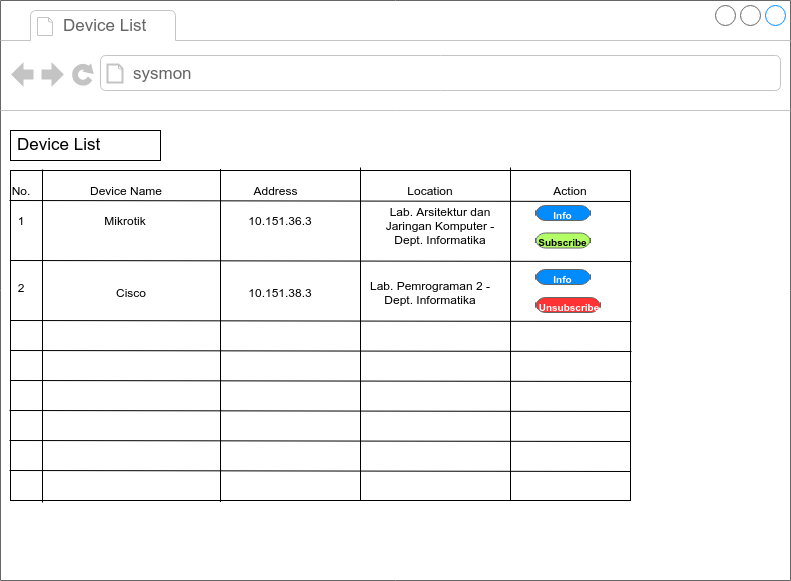
\includegraphics[width=9cm]{Images/C-3/antarmuka1.png}
        		\caption{Desain Antarmuka Menampilkan Daftar Perangkat Yang Tersedia}
        		\label{desain:antarmuka1}
        	\end{figure}
        
        	Desain antarmuka untuk menampilkan rincian dari antarmuka terkait dapat dilihat pada gambar \ref{desain:antarmuka2}. pada halaman ini pengguna dan pengolola dapat melihat seluruh rincian data yang ada pada perangkat. mulai dari nama perangkat, tipe perangkat, alamat perangkat, lokasi perangkat dan info apa saja yang dapat dipantau memalui OID.
        	
        	Pada halaman ini pengguna dan pengelola juga dapat belangganan dengan cara menekan sebuah tombol. tidak hanya berlangganan perangkatnya saja, pengguna dan pengelola juga dapat memilih untuk berlangganan info apa saja yang ingin didapatkan dari perangkat tersebut.
	        \begin{figure}[H]
	        	\centering
	        	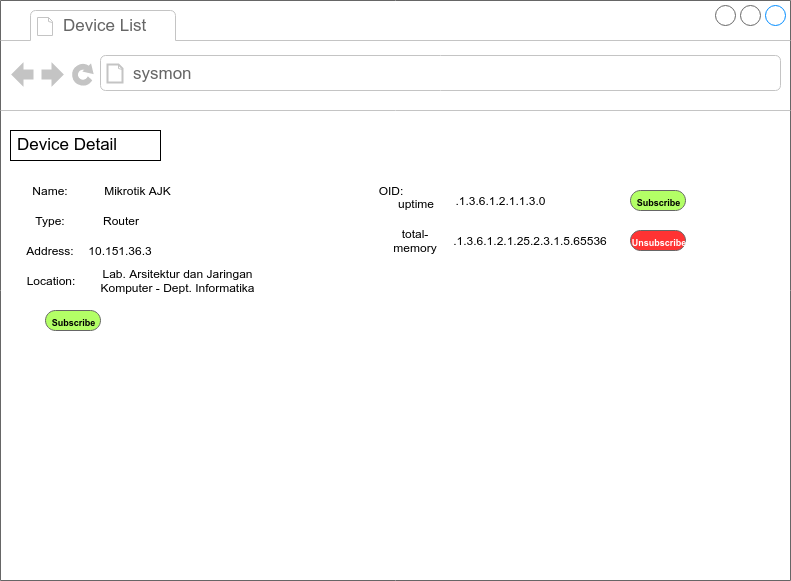
\includegraphics[width=9cm]{Images/C-3/antarmuka2.png}
	        	\caption{Desain Antarmuka Menampilkan Rincian dari Perangkat Terkait}
	        	\label{desain:antarmuka2}
	        \end{figure}
        
        	Desain antamuka pemantauan pernangkat dapat dilihat pada gambar \ref{desain:antarmuka3}. pada halaman ini, pengguna dan pengelola akan mendapatkan data dari seluruh perangkat yang sudah dilanggani. data yang ditampilkan pada halaman ini dipilih berdasarkan info yang dipilih pada antarmuka menampilkan rincian dari antarmuka terkait yang bisa dilihat pada gambar \ref{desain:antarmuka2}.
		    \begin{figure}[H]
		    	\centering
		    	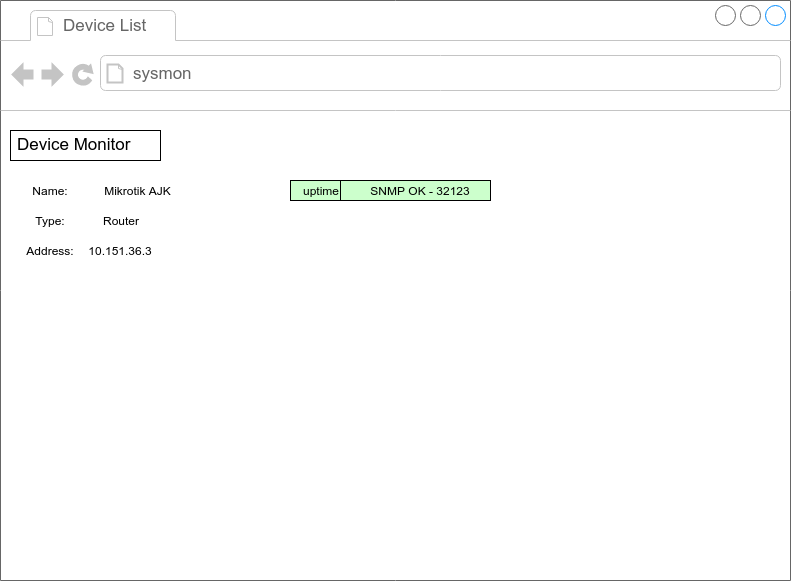
\includegraphics[width=9cm]{Images/C-3/antarmuka3.png}
		    	\caption{Desain Antarmuka Pemantauan Perangkat}
		    	\label{desain:antarmuka3}
		    \end{figure}
